\documentclass[a4paper,12pt,singlespacing]{article}
\usepackage[left=2.5cm,right=2.5cm,top=2.5cm]{geometry}
\usepackage[hyphens]{url}
\usepackage[backend=biber,style=alphabetic,backref=true,citecounter=true,citestyle=authoryear]{biblatex}
\usepackage[utf8]{inputenc}
\usepackage[T1]{fontenc}
\usepackage{csquotes}
\usepackage{hyperref}
\usepackage{setspace}
\usepackage{csquotes}
\usepackage[ngerman]{babel}
\usepackage{color}
\usepackage{hyperref}
\usepackage{pdflscape}
\usepackage{graphicx}
\usepackage{listings}
\usepackage{longtable}
\usepackage{array}
\usepackage{fancyhdr}
\addbibresource{cites.bib}
\pagestyle{empty}
\author{Andreas Lorer}

\chardef\_=`_

\graphicspath{{images/}
}\setlength{\parindent}{0ex}

% https://tex.stackexchange.com/questions/16765/biblatex-author-year-square-brackets
\newrobustcmd*{\parentexttrack}[1]{%
  \begingroup
  \blx@blxinit
  \blx@setsfcodes
  \blx@bibopenparen#1\blx@bibcloseparen
  \endgroup}

\AtEveryCite{%
  \let\parentext=\parentexttrack%
  \let\bibopenparen=\bibopenbracket%
  \let\bibcloseparen=\bibclosebracket}


\definecolor{materialGrey}{rgb}{0.27,0.27,0.27}
\definecolor{materialGreen}{rgb}{0.0, 0.8, 0.6}
\definecolor{materialRed}{rgb}{0.82, 0.1, 0.26}
\definecolor{materialYellow}{rgb}{1.0, 0.5, 0.0}
\definecolor{materialBlue}{rgb}{0.0, 0.5, 1.0}
\definecolor{lightgray}{rgb}{.9,.9,.9}
\definecolor{darkgray}{rgb}{.4,.4,.4}
\definecolor{purple}{rgb}{0.65, 0.12, 0.82}

\begin{document}
  % document styles for listings
  \lstset{
    backgroundcolor=\color{white},
    basicstyle=\footnotesize\ttfamily,
    breakatwhitespace=true,
    breaklines=true,
    numbers=left,
    numbersep=5pt,
    deletekeywords={event}, 
    numberstyle=\tiny,
    showspaces=false,
    showtabs=false,
    language=html,
    keywordstyle=\bfseries\color{materialRed},
    commentstyle=\itshape\color{materialGreen},
    columns=fullflexible,
    xleftmargin=0.5cm,
    xrightmargin=1cm,
    frame=lr,
    framesep=8pt,
    framerule=0pt
  }

% code listing support for javascript language
\lstdefinelanguage{JavaScript}{
  keywords={typeof, new, true, false, catch, function, return, null, catch, switch, var, if, in, while, do, else, case, break, length},
  keywordstyle=\color{materialBlue}\bfseries,
  ndkeywords={class, export, boolean, throw, implements, import, this},
  ndkeywordstyle=\color{darkgray}\bfseries,
  identifierstyle=\color{black},
  sensitive=false,
  comment=[l]{//},
  morecomment=[s]{/*}{*/},
  commentstyle=\color{purple}\ttfamily,
  stringstyle=\color{materialRed}\ttfamily,
  morestring=[b]',
  morestring=[b]"
}

\lstset{
   language=JavaScript,
   backgroundcolor=\color{lightgray},
   extendedchars=true,
   basicstyle=\footnotesize\ttfamily,
   showstringspaces=false,
   showspaces=false,
   numbers=left,
   numberstyle=\footnotesize,
   numbersep=9pt,
   tabsize=2,
   breaklines=true,
   showtabs=false,
   captionpos=b
}
\lstset{literate=%
   *{0}{{{\color{materialYellow}0}}}1
    {1}{{{\color{materialYellow}1}}}1
    {2}{{{\color{materialYellow}2}}}1
    {3}{{{\color{materialYellow}3}}}1
    {4}{{{\color{materialYellow}4}}}1
    {5}{{{\color{materialYellow}5}}}1
    {6}{{{\color{materialYellow}6}}}1
    {7}{{{\color{materialYellow}7}}}1
    {8}{{{\color{materialYellow}8}}}1
    {9}{{{\color{materialYellow}9}}}1
}
	%Coversheet
  \newcommand{\headline}{Real-Time Traffic Map Visualization}
  \newcommand{\subheadline}{Subtitle}
	%!TEX root = ../main.tex
% if you are not working with sublime text's latextools you can delete the previous line

\begin{titlepage}
  \sffamily
  \setlength{\tabcolsep}{0mm}
  \begin{tabular*}{\textwidth}{l@{\extracolsep\fill}r} 

  %\hspace{-0.4cm}
  
\includegraphics[width=5cm]{coversheet/images/dummyLogo.png} 
    &
  \raisebox{3mm}{
  \begin{tabular}{r}
    \rule{0cm}{0.5cm}
    Studiengang Angewandte Informatik\\[0.5mm]
    Fakultät Elektrotechnik und Informatik \\
  \end{tabular}}
  \end{tabular*}
  \setlength{\tabcolsep}{6pt}

  \vspace*{2cm}
  \begin{center}
      \textbf{\Large{Real-Time Traffic Map Visualization}}\\[1cm]
    \begin{doublespace}
      \textbf{\LARGE{Subtitle}}\\[1cm]
    \end{doublespace}
    
\includegraphics[width=0.5\textwidth]{coversheet/images/dummyLogo.png}\\[0.5cm]
    \vspace*{1cm}
    % \vspace*{2cm}
    \large{zur Erlangung des akademischen Grades}\\[2mm]
    \large{Bachelor of Science}\\
  \end{center}

  %\vfill
  \vspace{0.5cm}
  \begin{center}

  vorgelegt von:\\[5mm]
  {\Large Andreas Lorer} \\[5mm]
    Your Street\\
    Your Location\\
    \today \\[2cm]
  {\normalsize
    \begin{tabular}{rl}
    Prof. Name 1 \\
    Prof. Name 2\\
    \end{tabular}
  }
  \end{center}
  \vfill
\end{titlepage}


	%Table of contents
  \thispagestyle{empty}
	\tableofcontents 
  \clearpage
  \pagestyle{fancy}
  \fancyhf{}
  % \rhead{}
  \lhead{Subtitle}
  \rfoot{\thepage}
  \renewcommand{\headrulewidth}{0.4pt}
  \renewcommand{\footrulewidth}{0.4pt}

  \begin{newpage}
	
	\section{Einleitung}
		
	\label{sec:Einleitung}
	 %  Data can be rather complex. To understand complex systems we have different approaches in our professions. In software development we have tools like "Divide and Conquer" to help us break things into smaller pieces. But what if that does not help us understanding the fundamental underlying principles. Bret Victor describes in his essay "Up and Down the Ladder of Abstraction" a more visual approach for finding a profound insight into complex systems: 

	 %  \begin{quote}
		% 	\emph{"`When designing [a system], the challenge lies not in constructing the system, but in understanding it. In the absence of theory, we must develop an intuition to guide our decisions. The design process is thus one of exploration and discovery."'} \parencite{victor}
		% \end{quote}

	 %  Data is often coupled to each other. Separating it into smaller junks can alter its meaning, because the context could get lost or changed. Often times interesting datasets are described interesting especially because they have relations that tell a story. Thats why data visualization got so popular in this decade. We searched for new exciting ways of exploring data and tell untold stories. Especially on maps we are seeing all kinds of neat visualizations, giving data a geospatial context. Ranging from demographic health coverage, crime rates, earthquake data for different regions to a live aircraft flight radar.

		% Visualizations help us to understand complex topics in a more consumable way. They enable us to explore data, exposing twists and secrets that otherwise might have been left buried in that huge pile that data often times is.\\

		Datenvisualisierung ist ein Thema, das nicht nur in jüngster Zeit sehr viel Zuwendung fand, sondern auch zur Analyse von Sachverhalten immer wichtiger wird. So lassen sich komplexe Zusammenhänge eines Systems, oftmals erst dann richtig begreifen, wenn wir alle möglichen Zustände davon erfassen können. In "`Up and Down the Ladder of Abstraction"', beschreibt Bret Victor wie sich Systeme in ihrer Ganzheit besser begreifen und gestalten lassen.

		\begin{quote}
			\emph{"`When designing [a system], the challenge lies not in constructing the system, but in understanding it. In the absence of theory, we must develop an intuition to guide our decisions. The design process is thus one of exploration and discovery."'} \parencite{victor}
		\end{quote}

		Auch eine Ansammlung an Daten ist erst einmal sehr abstrakt. In einer Datenbank in Relation gebracht, bleiben die meisten Erkenntnisse und Stories verborgen. Ein tieferes Verständnis, begreifen wir erst dann, wenn wir sie auswerten. Die Art der Datenvisualisierung hat sich in den letzten Jahren stark gewandelt. Während anfangs vor allem Daten in der Form von Häufigkeitsanalysen ausgewertet und als Bar- oder Linechart visualisiert wurden, haben wir heute interaktive Karten um geospartiale Zusammenhänge zu veranschaulichen.

		Diesen Trend von dynamischen Visualisierungen nahmen auch verschiedene namhafte Verkehrsunternehmen auf und wir sahen eine Reihe von Live Karten ans Netz gehen. Zum Beispiel der Fligt-Radar\footnote{\url{https://www.flightradar24.com/}} für Flugzeuge, Marinetraffic-Map\footnote{\url{https://www.marinetraffic.com/}} in der Schifffahrt oder auch für die Live Simulation von Wetterdaten\footnote{\url{https://mapbox.github.io/webgl-wind/demo/}}. 

		Auch regional gibt es verschiedene Produkte die veröffentlicht wurden. Beispielsweise der Zugradar\footnote{\url{http://bahn.de/zugradar}} (2014) und der Busradar\footnote{\url{https://play.google.com/store/apps/details?id=de.hafas.android.dbbusradar}} der Deutschen Bahn oder eine Karte für das S-Bahn Netz in München\footnote{\url{http://s-bahn-muenchen.hafas.de/}} (2009).

		Eine gesamte Erfassung des öffentlichen Verkehrs ging ebenfalls 2014 mit Travic\footnote{\url{http://tracker.geops.de/}}\label{travic} online und bietet mit über 650 integrierten Fahrplänen eine enorme Abdeckung. Da die Live Karten der Deutschen Bahn damals nur die Visualisierung der eigenen Bus und Bahnlinien ermöglichte, war Travic darin bestrebt diese Lücke zu schließen und den gesamten öffentlichen Verkehr darzustellen. 
		Zusätzlich sei noch LiveMap24 \footnote{\url{https://www.livemap24.com/}} von Verdict erwähnt. Auch eine Live Karte, deren Veröffentlichungsdatum mir allerdings nicht bekannt ist.

		Der Vorteil einer Digitalen Karte besteht in seiner ständigen Aktualität. Ein statischer Fahrplan kann keine Informationen zu Störungen, Verspätungen oder Ausfall eines Zuges geben. Auf einer Live Karte lassen sich solche Informationen visuell aufbereiten und dem Anwender über die Benutzeroberfläche vermitteln. Der Betrachter kann sehen wie viele Fahrzeuge gerade aktiv sind und kann zusätzlich zum statischen Fahrplan auch visuell erleben wo sich sein Zug oder Bus befindet. 
		Da gleichzeitig Fahrplan als auch Karte vorhanden sind, ist auch eine geographische Orientierung möglich. \emph{"`Der Zug hat 5 Minuten Verspätung"'} wird ein visueller Kontext gegeben und ist dadurch nicht mehr nur eine Aussage, sondern erfahrbar.
    Einen Nutzen in einer Live Karte sehen aber nicht nur Pendler oder Reisende, sondern auch Verkehrsunternehmen, Städte oder Verkehrsforscher.\\
		
		%Durch die erstell... lassen sich Erkenntnisse gewinnen, die durch diese Form der Visualisierung Einblicke ermöglichen, die durch eine gedruckte 2D Karte in dieser Art, nicht möglich gewesen währen.\\

		Diese Arbeit befasst sich umfassend mit der Entwicklung einer Live Karte für den öffentlichen Nahverkehr anhand von GTFS Daten. Der Fokus liegt dabei in der Gestaltung von verschiedenen Visualisierungen, welche die User Experience erhöhen und die Karte nicht nur interaktiv, sondern vor allem auch dem Benutzer Freude bei der Bedienung bereitet.

		% Aufzählen der eigenen Features der Karte. Was für Sachen wurden entworfen etc.

		% Aufzählen was in den einzelnen Kapiteln noch alles behandelt wird.

		% MOTIVATION (Recherche für Moovel um .... (was soll diese Arbeit herausfinden))

		% Abstract: https://www.researchgate.net/publication/224581089_ICE_-_Visual_analytics_for_transportation_incident_datasets

	% section einleitung

\end{newpage}
  \begin{newpage}
  \section{Related Work}
  \label{sec:related_work}
    Es existieren mehrere Publikationen, welche für diese Arbeit Relevanz haben oder die für dieses Thema wertvolle Informationen bereitgestellt haben. Die wichtigsten werden in diesem Abschnitt vorgestellt.\\

    Einen ersten guten Überblick zum momentanen Stand von Transportvisualisierungen bietet das Paper \textit{"`Visualizing Public Transport Systems: State-of-the-Art and Future Challenges"'}\parencite{marchi} von Massimo De Marchi. In seiner Arbeit wird dargelegt, welche visuellen Lösung bereits bestehen und welche stärken / schwächen sie haben. Dabei wird auf Zwei unterschiedliche Benutzertypen eingegangen. Namentlich als "`Traveler"' und "`Transportation Researcher"' genannt. Er beschreibt dabei welche verschiedenen Eigenschaften die jeweilige Nutzerrolle besitzt und welche Bedürfnisse diese haben. Diese Frage \textit{"`Wer soll die interaktive Karte am ende benutzen?"'} ist auch bei der Erstellung dieser Arbeit von entscheidender Bedeutung gewesen. Je nach Typ bedarf es einem anderen Schwerpunkt gerecht zu werden. In dieser Arbeit sollen vor allem diejenigen einen Nutzen daraus ziehen können, die\\

    \parencite{mbtaviz} beschreibt sehr gut die Vorgehensweise und verwendeten Technologien für die Umsetzung der Visualisierung von \textit{"`An interactive exploration of Boston's subway system"'}\footnote{\url{http://mbtaviz.github.io/}}. Es werden dabei sowohl die verwendeten Tools beschrieben als auch Mockups gezeigt die eindrücke in den Arbeitsprozess gewähren. Die resultierenden Visualisierungen und deren Detailgrad sind sehr Eindrucksvoll und lassen einen tiefen Einblick in das Verkehrsnetz zu.\\

    Eine weitere wertvolle Quelle ist die Arbeit von Patrick Brosi \textit{"`Real-Time Movement Visualization of Public Transit Data"'}\parencite{brosi}. Brosi stellt dabei die Entwicklung von Travic vor, der bereits eingangs\footnote{siehe Kapitel~\ref{travic}} erwähnt wurde. Seine Arbeit zeigt einen Lösungsweg für die Visualisierung von Tausenden Fahrzeugen auf einer interaktiven Karte. Interessant sind dabei die diskutierten Vor- und Nachteile von verschiedenen Lösungsansätzen.
    Während seine Arbeit keine Datenbank verwendet, sondern alle Daten in den RAM-Speicher des Servers läd, um schnelle Zugriffszeiten zu erreichen, soll in unserer Arbeit eine Postgresql Datenbank zum Einsatz kommen. 
    Auch hat unsere Arbeit nicht den Anspruch eine weltweite Live Karte zur Verfügung zu stellen, sondern fokussiert sich lediglich auf den Raum Stuttgart unter Verwendung eines GTFS Feeds des Verkehrsverbundes Stuttgart-VVS. 
    Der Kern der Arbeit beschäftigt sich tiefer mit dem finden von neuen Visualisierungsansätzen und UI-Komponenten. Es steht also nicht die Entwicklung eines fertigen Produkts im Vordergrund, sondern viel mehr darum, wie Nutzern auf visuellem Weg Informationen auf interessante Weise präsentieren werden können.

  % sec:related_work (end)

\end{newpage}
  %!TEX root = ../main.tex

\begin{newpage}
	
	\section{Grundlagen}
	\label{sec:Grundlagen}

	\subsection{Das GTFS Datenformat}
	\label{ssec:das_gtfs_datenformat}
		Das GTFS (General Transit Feed Specification) ist eine Datenstandardisierung die von Google im Jahr 2006 entwickelt wurde. Vor dessen Einführung gab es weder eine einheitliche Standardisierung, noch ein "`de facto Standard"' für die Fahrpläne des Öffentlichen Nahverkehrs in den USA. GTFS ermöglichte es Transit Organisationen ihre Daten für dritte zu öffnen und ist heute das weit verbreitetste offene Datenformat für den öffentlichen Nahverkehr.\parencite[S. 2]{roush}\\

    Ein GTFS Feed besteht aus mindestens 6 und maximal 13 \texttt{csv-Dateien}, die im \texttt{.txt} Format vorliegen müssen. Die Struktur eines Feeds lässt sich in Worten wie folgt beschreiben:

    \begin{quote}
      \textit{Ein GTFS Feed besteht aus einer oder mehreren Routen. Jede Route (\texttt{routes.txt}) hat einen oder mehrere Trips (\texttt{trips.txt}). Jeder Trip besucht eine Abfolge von Stops (\texttt{stops.txt}) zu einer bestimmten Zeit (\texttt{stop\_times.txt}). Trips und Stop-Zeit beinhalten nur die Tageszeit Informationen. Der Kalender (calendar.txt und \texttt{calendar\_dates.txt}) bestimmt dann, an welchen Tagen ein bestimmter Trip stattfindet.} \parencite[S. 8]{zervaas}
    \end{quote}

		Vor allem für digitale Produkte, wie zum Beispiel Trip-Planer, die viele verschiedene Fahrpläne von unterschiedlichen Unternehmen in ihren Service integrieren müssen, ist ein standardisiertes Datenformat unbedingt notwendig. 
		Ansonsten müsste jede App die Entwickelt wird, auf das Datenformat der jeweiligen Verkehrsunternehmen angepasst werden. Das wiederum bedeutet, dass je nach Implementierung innerhalb dieser Unternehmen, die Datenformate gänzlich voneinander abweichen können. Für jeden dieser Anbieter müsste folglich eine ganz eigene Datenverarbeitungslogik geschrieben werden.
    Darüber hinaus könnte natürlich jedes Verkehrsunternehmen jederzeit sein eigenes Datenformat ändern, was zur Folge hat, dass ein App-Entwickler diese Änderungen auch in sein Produkt übernehmen muss. Bei einer Integration von Daten, aus beliebig vielen unterschiedlichen Verkehrsunternehmen (Beispiel: Trip-Planer für ein ganzes Land), könnten sich laufend Änderungen ergeben die integriert werden müssen, oder das eigene Produkt würde nicht mehr zuverlässig funktionieren. Dies übersteigt die Wartbarkeit und Robustheit einer App, denn sie würde möglicherweise immer dann nicht mehr funktionieren, wenn ein Dritter entscheidet sein eigenes Datenformat zu ändern. Aus diesem Grund gab es bis vor einiger Zeit nahezu keine Trip oder Routen-Planer Anwendungen die nicht von den Verkehrsunternehmen selbst stammten würden. Der Status Quo war: Jedes Verkehrsunternehmen hat seine eigene Anwendung für die Fahrplanauskunft. Unter anderem aus diesem Grund erfolge die Adaption an das neue GTFS Format sehr schnell und so sind heute die meisten öffentlich verfügbaren Fahrpläne im GTFS Format auf Plattformen wie: \url{http://transitfeeds.com} oder \url{https://transit.land/} frei verfügbar.\footnote{Momentan besitzt Transitfeeds 535 Feeds (Stand 18.08.2017)}\\

    Trotz der Standardisierung durch GTFS gibt es immer noch diverse Freiräume in der Umsetzung des Formats. Wie anfangs erwähnt wurde, beträgt die Anzahl der Dateien die für ein gültiges GTFS Feed benötigt werden nur Sechs. Es sind allerdings bis zu 13 Dateien möglich. Dies zeigt wie viele unterschiedliche Informationen ein GTFS Feed bereitstellen kann, aber nicht muss. 
    Auch innerhalb der Dateien gibt es Felder die vorhanden sein "`müssen"' oder nur "`dürfen"'. Beispielsweise muss das Feld \texttt{route\_short\_name} in \texttt{routes.txt} vorhanden sein, aber \texttt{route\_desc} (Route Description) nicht. Der Interpretationsspielraum lässt sich aber noch weiter veranschaulichen, wenn wir uns Tabelle ~\ref{table:gtfs_differences} ansehen. In dieser Tabelle sind Zwei Einträge aus unterschiedlichen GTFS Feeds aufgelistet.
    Wir sehen, dass die Spalte \texttt{route\_id} bei Stuttgart-VVS als Zahlenwert angegeben wird, wohingegen Boston-MBTA einen Text verwendet.

    \begin{longtable}{|>{\raggedright \arraybackslash}p{3.0cm}|>{\raggedright \arraybackslash}p{2.0cm}|>{\raggedright \arraybackslash}p{3.5cm}|>{\raggedright \arraybackslash}p{5.5cm}|}
    \caption{Unterschiede innerhalb GTFS} 
    \label{table:gtfs_differences}\\
      \hline
       & route\_id & route\_short\_name & route\_long\_name\\
      \hline
      Stuttgart-VVS & 379 & U1 & Fellbach - Hauptbahnhof - Vaihingen\\
      \hline
      Boston-MBTA & Blue Line & Blue & Bowdoin - Wonderland\\
      \hline
    \end{longtable}

    % Die fehlende/nicht gegebene Übereinstimmung beim Gebrauch der Variablen führt als zu Problemen bei der ...

    "`Blue Line"' ist dabei die Bezeichnung der U-Bahnlinie\parencite{wiki_blue_line}. Wir sehen also, dass Stuttgart-VVS die \texttt{route\_id} zur eindeutigen Identifizierung mittels Zahlenwert verwendet wohingegen Boston-MBTA dieses Feld nutzt, um den Namen der Linie zu beschreiben. Angenommen wir verwenden die \texttt{route\_id} in einer Benutzeroberfläche wie in Abbildung ~\ref{fig:gtfs_differences}.

    \begin{figure}[htbp]
      \begin{center}
        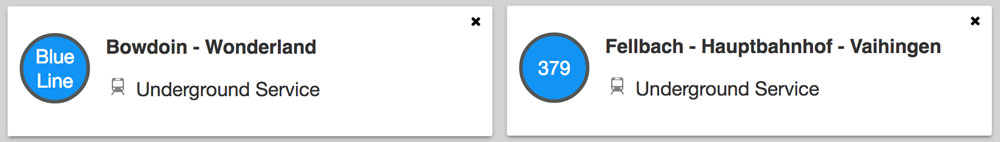
\includegraphics[width=\textwidth]{gtfs_differences.jpg}
        \caption{UI Element mit GTFS Informationen}
        \label{fig:gtfs_differences}
      \end{center}
    \end{figure}

    Links in der Abbildung ist die Korrekte Bezeichnung der Route zu sehen nämlich "Blue Line", wohingegen rechts nur eine numerische ID zu sehen ist, die nicht für den Nutzer vorgesehen und damit falsch ist. Damit die rechte Seite korrekt wäre müsste dort \texttt{U1} abgebildet sein. Die fehlende beziehungsweise nicht gegebene Übereinstimmung der beiden Feeds führt also zu Problemen bei der Darstellung die auch durch die Verwendung eines anderen Feldes wie zum Beispiel \texttt{route\_short\_name} nicht behoben werden können.\\

		Da das GTFS-Format das grundlegende Datenformat für diese Arbeit ist, sollen nachfolgend kurz die wichtigsten Tabellen beschrieben werden.

		\begin{itemize}
			\item \texttt{agency.txt}: Beinhaltet Informationen über die Verkehrsunternehmen, welche das Feed und die Daten bereitstellen.

			\item \texttt{routes.txt}: Eine Route ist eine Gruppierung von Trips. Die verschiedenen Eigenschaften einer Route werden in dieser Tabelle gespeichert.

			\item \texttt{trips.txt}: Ein Trip gehört zu einer Route. Eine Route kann dabei beliebig viele Trips haben. Welche Trips aktiv sind wird durch den Kalender festgelegt.

			\item \texttt{calendar.txt}: Bestimmt, an welchen Tagen ein Trip aktiv ist.

			\item \texttt{stop\_times.txt}: Diese Tabelle beschreibt welche Stationen nacheinander angefahren werden. Für jede Station beinhaltet sie die Ankunfts- und Abfahrtszeiten.

			\item \texttt{stops.txt}: Stellt nähere Informationen für jede Station zur Verfügung wie zum Beispiel den Stationsnamen und deren Position.

			\item \texttt{shapes.txt}: Jeder Trip kann eine dazugehörigen Polyline\footnote{Linienverlauf} haben. Eine Polyline ist dabei nichts anderes als eine Abfolge von Punkten, die, wenn man sie verbindet, eine Linie ergeben. Um einen Routenverlauf auf eine Karte zu zeichnen, wird diese Tabelle folglich unbedingt benötigt. 
		\end{itemize}

	\section{Existierende Projekte}
	\label{sec:existierende_projekte}

\end{newpage}
% section grundlagen
  \begin{newpage}
	% \hline
	\vspace*{\fill}
	\section*{Eidesstattliche Erklärung }
	Hiermit versichere ich, die vorliegende Arbeit selbstständig und unter ausschließlicher Verwendung der angegebenen Literatur und Hilfsmittel erstellt zu haben. Die Arbeit wurde bisher, in gleicher oder ähnlicher Form, keiner anderen Prüfungsbehörde vorgelegt und auch nicht veröffentlicht.\\

	\vspace{3cm}
	\begin{tabular*}{\textwidth}{c@{\extracolsep\fill}cc}
	\cline{1-1}
	\cline{3-3}
	\\
	\ \ \ \ \ \ \ \ \ Unterschrift \ \ \ \ \ \ \ \ \ \ & & \ \ \ \ \ \ \ \ \ Ort, Datum \ \ \ \ \ \ \ \ \ \\
	\end{tabular*}
\end{newpage}

\newpage
	\pagebreak
  
	\printbibliography

\end{document}